\documentclass[1p]{elsarticle_modified}
%\bibliographystyle{elsarticle-num}

%\usepackage[colorlinks]{hyperref}
%\usepackage{abbrmath_seonhwa} %\Abb, \Ascr, \Acal ,\Abf, \Afrak
\usepackage{amsfonts}
\usepackage{amssymb}
\usepackage{amsmath}
\usepackage{amsthm}
\usepackage{scalefnt}
\usepackage{amsbsy}
\usepackage{kotex}
\usepackage{caption}
\usepackage{subfig}
\usepackage{color}
\usepackage{graphicx}
\usepackage{xcolor} %% white, black, red, green, blue, cyan, magenta, yellow
\usepackage{float}
\usepackage{setspace}
\usepackage{hyperref}

\usepackage{tikz}
\usetikzlibrary{arrows}

\usepackage{multirow}
\usepackage{array} % fixed length table
\usepackage{hhline}

%%%%%%%%%%%%%%%%%%%%%
\makeatletter
\renewcommand*\env@matrix[1][\arraystretch]{%
	\edef\arraystretch{#1}%
	\hskip -\arraycolsep
	\let\@ifnextchar\new@ifnextchar
	\array{*\c@MaxMatrixCols c}}
\makeatother %https://tex.stackexchange.com/questions/14071/how-can-i-increase-the-line-spacing-in-a-matrix
%%%%%%%%%%%%%%%

\usepackage[normalem]{ulem}

\newcommand{\msout}[1]{\ifmmode\text{\sout{\ensuremath{#1}}}\else\sout{#1}\fi}
%SOURCE: \msout is \stkout macro in https://tex.stackexchange.com/questions/20609/strikeout-in-math-mode

\newcommand{\cancel}[1]{
	\ifmmode
	{\color{red}\msout{#1}}
	\else
	{\color{red}\sout{#1}}
	\fi
}

\newcommand{\add}[1]{
	{\color{blue}\uwave{#1}}
}

\newcommand{\replace}[2]{
	\ifmmode
	{\color{red}\msout{#1}}{\color{blue}\uwave{#2}}
	\else
	{\color{red}\sout{#1}}{\color{blue}\uwave{#2}}
	\fi
}

\newcommand{\Sol}{\mathcal{S}} %segment
\newcommand{\D}{D} %diagram
\newcommand{\A}{\mathcal{A}} %arc


%%%%%%%%%%%%%%%%%%%%%%%%%%%%%5 test

\def\sl{\operatorname{\textup{SL}}(2,\Cbb)}
\def\psl{\operatorname{\textup{PSL}}(2,\Cbb)}
\def\quan{\mkern 1mu \triangleright \mkern 1mu}

\theoremstyle{definition}
\newtheorem{thm}{Theorem}[section]
\newtheorem{prop}[thm]{Proposition}
\newtheorem{lem}[thm]{Lemma}
\newtheorem{ques}[thm]{Question}
\newtheorem{cor}[thm]{Corollary}
\newtheorem{defn}[thm]{Definition}
\newtheorem{exam}[thm]{Example}
\newtheorem{rmk}[thm]{Remark}
\newtheorem{alg}[thm]{Algorithm}

\newcommand{\I}{\sqrt{-1}}
\begin{document}

%\begin{frontmatter}
%
%\title{Boundary parabolic representations of knots up to 8 crossings}
%
%%% Group authors per affiliation:
%\author{Yunhi Cho} 
%\address{Department of Mathematics, University of Seoul, Seoul, Korea}
%\ead{yhcho@uos.ac.kr}
%
%
%\author{Seonhwa Kim} %\fnref{s_kim}}
%\address{Center for Geometry and Physics, Institute for Basic Science, Pohang, 37673, Korea}
%\ead{ryeona17@ibs.re.kr}
%
%\author{Hyuk Kim}
%\address{Department of Mathematical Sciences, Seoul National University, Seoul 08826, Korea}
%\ead{hyukkim@snu.ac.kr}
%
%\author{Seokbeom Yoon}
%\address{Department of Mathematical Sciences, Seoul National University, Seoul, 08826,  Korea}
%\ead{sbyoon15@snu.ac.kr}
%
%\begin{abstract}
%We find all boundary parabolic representation of knots up to 8 crossings.
%
%\end{abstract}
%\begin{keyword}
%    \MSC[2010] 57M25 
%\end{keyword}
%
%\end{frontmatter}

%\linenumbers
%\tableofcontents
%
\newcommand\colored[1]{\textcolor{white}{\rule[-0.35ex]{0.8em}{1.4ex}}\kern-0.8em\color{red} #1}%
%\newcommand\colored[1]{\textcolor{white}{ #1}\kern-2.17ex	\textcolor{white}{ #1}\kern-1.81ex	\textcolor{white}{ #1}\kern-2.15ex\color{red}#1	}

{\Large $\underline{12n_{0503}~(K12n_{0503})}$}

\setlength{\tabcolsep}{10pt}
\renewcommand{\arraystretch}{1.6}
\vspace{1cm}\begin{tabular}{m{100pt}>{\centering\arraybackslash}m{274pt}}
\multirow{5}{120pt}{
	\centering
	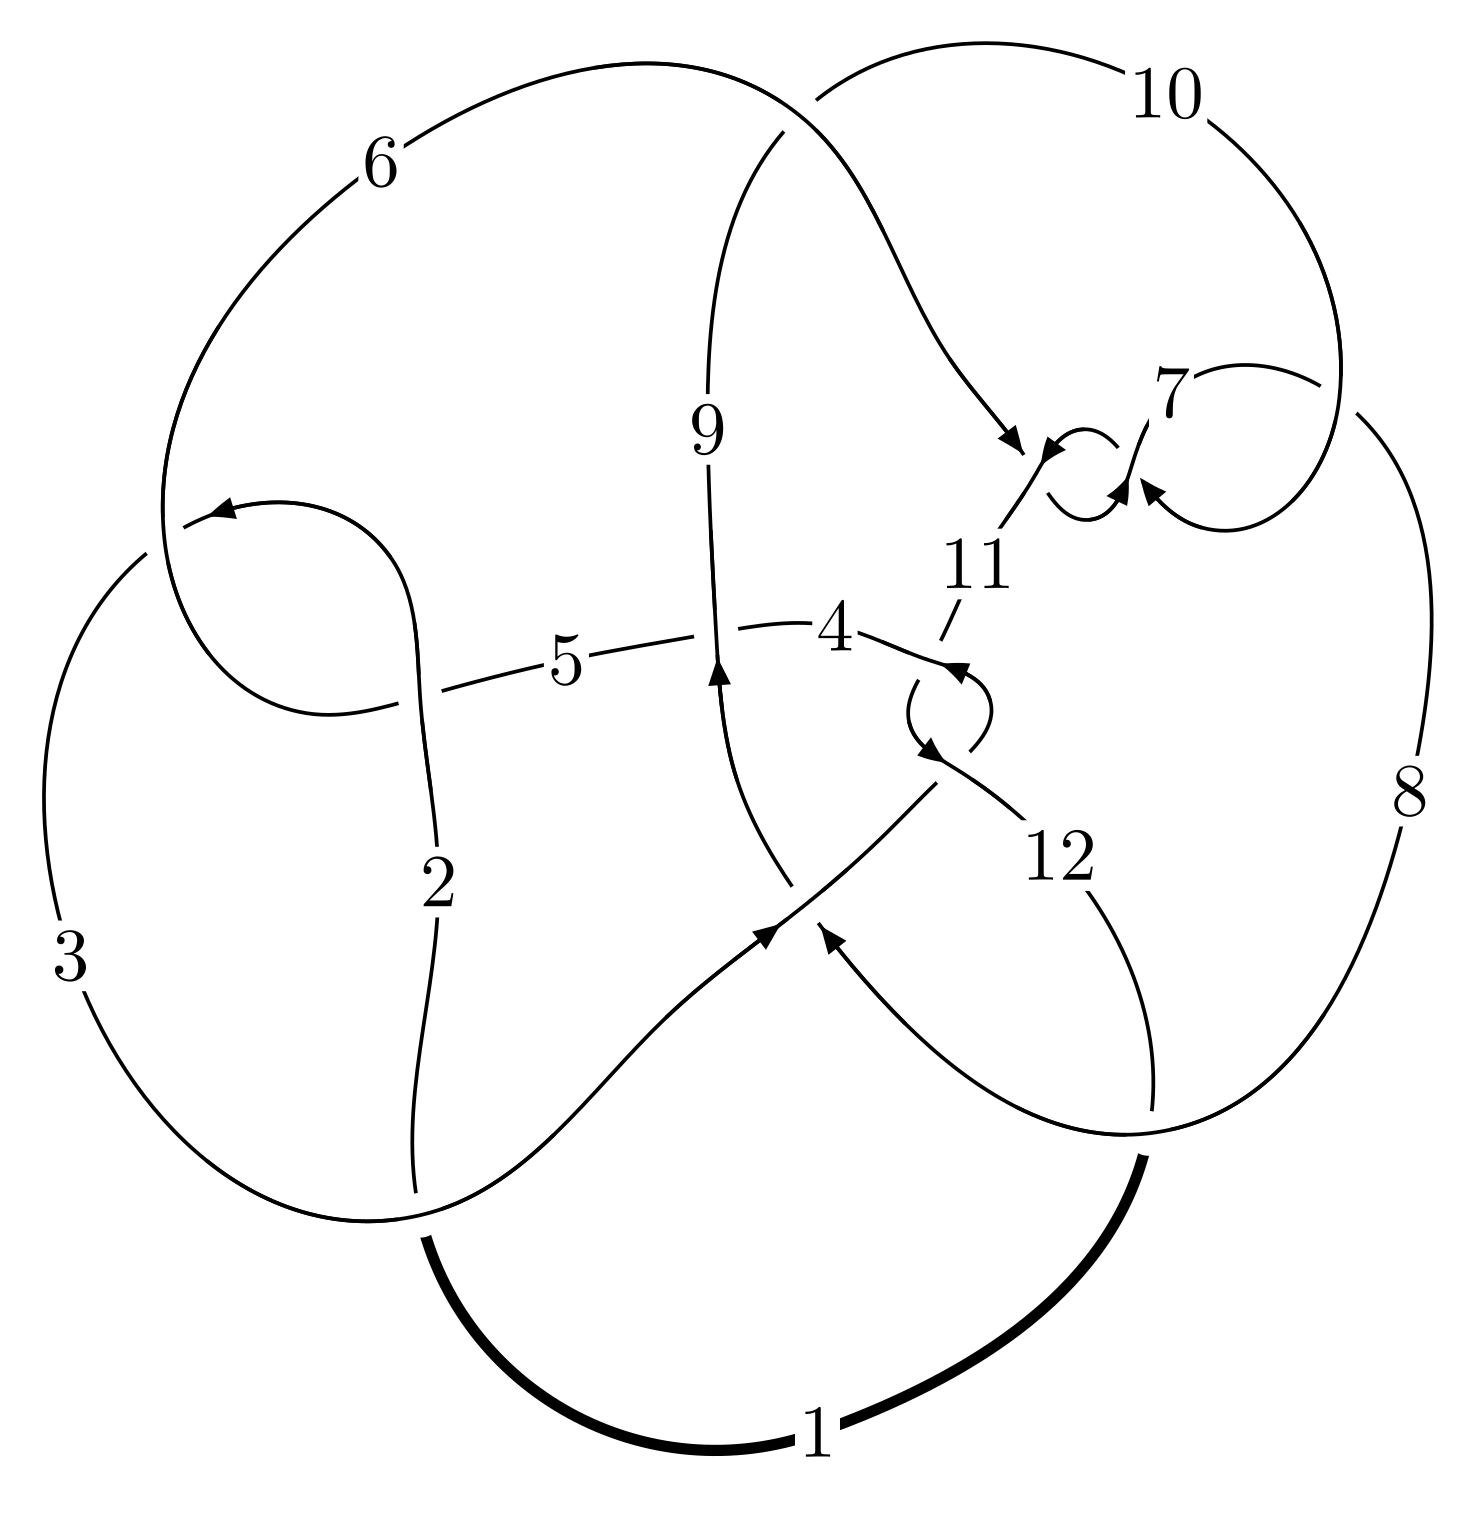
\includegraphics[width=112pt]{../../../GIT/diagram.site/Diagrams/png/2592_12n_0503.png}\\
\ \ \ A knot diagram\footnotemark}&
\allowdisplaybreaks
\textbf{Linearized knot diagam} \\
\cline{2-2}
 &
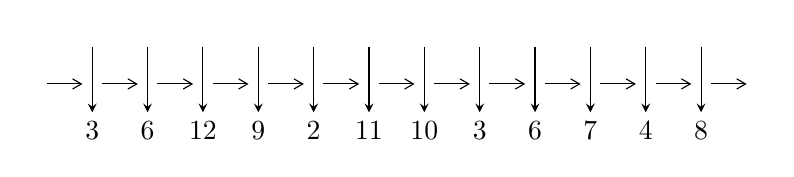
\begin{tikzpicture}[x=20pt, y=17pt]
	% nodes
	\node (C0) at (0, 0) {};
	\node (C1) at (1, 0) {};
	\node (C1U) at (1, +1) {};
	\node (C1D) at (1, -1) {3};

	\node (C2) at (2, 0) {};
	\node (C2U) at (2, +1) {};
	\node (C2D) at (2, -1) {6};

	\node (C3) at (3, 0) {};
	\node (C3U) at (3, +1) {};
	\node (C3D) at (3, -1) {12};

	\node (C4) at (4, 0) {};
	\node (C4U) at (4, +1) {};
	\node (C4D) at (4, -1) {9};

	\node (C5) at (5, 0) {};
	\node (C5U) at (5, +1) {};
	\node (C5D) at (5, -1) {2};

	\node (C6) at (6, 0) {};
	\node (C6U) at (6, +1) {};
	\node (C6D) at (6, -1) {11};

	\node (C7) at (7, 0) {};
	\node (C7U) at (7, +1) {};
	\node (C7D) at (7, -1) {10};

	\node (C8) at (8, 0) {};
	\node (C8U) at (8, +1) {};
	\node (C8D) at (8, -1) {3};

	\node (C9) at (9, 0) {};
	\node (C9U) at (9, +1) {};
	\node (C9D) at (9, -1) {6};

	\node (C10) at (10, 0) {};
	\node (C10U) at (10, +1) {};
	\node (C10D) at (10, -1) {7};

	\node (C11) at (11, 0) {};
	\node (C11U) at (11, +1) {};
	\node (C11D) at (11, -1) {4};

	\node (C12) at (12, 0) {};
	\node (C12U) at (12, +1) {};
	\node (C12D) at (12, -1) {8};
	\node (C13) at (13, 0) {};

	% arrows
	\draw[->,>={angle 60}]
	(C0) edge (C1) (C1) edge (C2) (C2) edge (C3) (C3) edge (C4) (C4) edge (C5) (C5) edge (C6) (C6) edge (C7) (C7) edge (C8) (C8) edge (C9) (C9) edge (C10) (C10) edge (C11) (C11) edge (C12) (C12) edge (C13) ;	\draw[->,>=stealth]
	(C1U) edge (C1D) (C2U) edge (C2D) (C3U) edge (C3D) (C4U) edge (C4D) (C5U) edge (C5D) (C6U) edge (C6D) (C7U) edge (C7D) (C8U) edge (C8D) (C9U) edge (C9D) (C10U) edge (C10D) (C11U) edge (C11D) (C12U) edge (C12D) ;
	\end{tikzpicture} \\
\hhline{~~} \\& 
\textbf{Solving Sequence} \\ \cline{2-2} 
 &
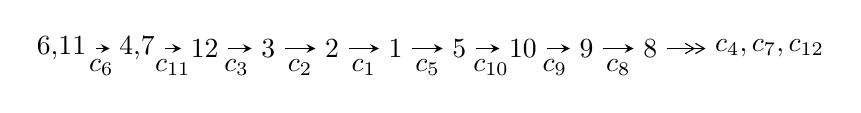
\begin{tikzpicture}[x=23pt, y=7pt]
	% node
	\node (A0) at (-1/8, 0) {6,11};
	\node (A1) at (17/16, 0) {4,7};
	\node (A2) at (17/8, 0) {12};
	\node (A3) at (25/8, 0) {3};
	\node (A4) at (33/8, 0) {2};
	\node (A5) at (41/8, 0) {1};
	\node (A6) at (49/8, 0) {5};
	\node (A7) at (57/8, 0) {10};
	\node (A8) at (65/8, 0) {9};
	\node (A9) at (73/8, 0) {8};
	\node (C1) at (1/2, -1) {$c_{6}$};
	\node (C2) at (13/8, -1) {$c_{11}$};
	\node (C3) at (21/8, -1) {$c_{3}$};
	\node (C4) at (29/8, -1) {$c_{2}$};
	\node (C5) at (37/8, -1) {$c_{1}$};
	\node (C6) at (45/8, -1) {$c_{5}$};
	\node (C7) at (53/8, -1) {$c_{10}$};
	\node (C8) at (61/8, -1) {$c_{9}$};
	\node (C9) at (69/8, -1) {$c_{8}$};
	\node (A10) at (11, 0) {$c_{4},c_{7},c_{12}$};

	% edge
	\draw[->,>=stealth]	
	(A0) edge (A1) (A1) edge (A2) (A2) edge (A3) (A3) edge (A4) (A4) edge (A5) (A5) edge (A6) (A6) edge (A7) (A7) edge (A8) (A8) edge (A9) ;
	\draw[->>,>={angle 60}]	
	(A9) edge (A10);
\end{tikzpicture} \\ 

\end{tabular} \\

\footnotetext{
The image of knot diagram is generated by the software ``\textbf{Draw programme}" developed by Andrew Bartholomew(\url{http://www.layer8.co.uk/maths/draw/index.htm\#Running-draw}), where we modified some parts for our purpose(\url{https://github.com/CATsTAILs/LinksPainter}).
}\phantom \\ \newline 
\centering \textbf{Ideals for irreducible components\footnotemark of $X_{\text{par}}$} 
 
\begin{align*}
I^u_{1}&=\langle 
u^7+u^6+3 u^5+2 u^4+2 u^3+2 u^2+b,\;a-1,\;u^8+u^7+4 u^6+3 u^5+5 u^4+4 u^3+u^2+3 u-1\rangle \\
I^u_{2}&=\langle 
- u^2+b+2 u,\;a+1,\;u^3- u^2+2 u-1\rangle \\
I^u_{3}&=\langle 
u^{15}+2 u^{14}+7 u^{13}+10 u^{12}+18 u^{11}+19 u^{10}+17 u^9+12 u^8-2 u^7-3 u^6-9 u^5-4 u^4+5 u^3+u^2+2 b+4 u+1,\\
\phantom{I^u_{3}}&\phantom{= \langle  }2 u^{17}+5 u^{16}+\cdots+2 a+19 u,\;u^{18}+3 u^{17}+\cdots+4 u+1\rangle \\
I^u_{4}&=\langle 
u^2 a- a u+b+u,\;u^2 a+a^2- a u+3 u^2+a- u+5,\;u^3- u^2+2 u-1\rangle \\
\\
\end{align*}
\raggedright * 4 irreducible components of $\dim_{\mathbb{C}}=0$, with total 35 representations.\\
\footnotetext{All coefficients of polynomials are rational numbers. But the coefficients are sometimes approximated in decimal forms when there is not enough margin.}
\newpage
\renewcommand{\arraystretch}{1}
\centering \section*{I. $I^u_{1}= \langle u^7+u^6+3 u^5+2 u^4+2 u^3+2 u^2+b,\;a-1,\;u^8+u^7+4 u^6+3 u^5+5 u^4+4 u^3+u^2+3 u-1 \rangle$}
\flushleft \textbf{(i) Arc colorings}\\
\begin{tabular}{m{7pt} m{180pt} m{7pt} m{180pt} }
\flushright $a_{6}=$&$\begin{pmatrix}1\\0\end{pmatrix}$ \\
\flushright $a_{11}=$&$\begin{pmatrix}0\\u\end{pmatrix}$ \\
\flushright $a_{4}=$&$\begin{pmatrix}1\\- u^7- u^6-3 u^5-2 u^4-2 u^3-2 u^2\end{pmatrix}$ \\
\flushright $a_{7}=$&$\begin{pmatrix}1\\u^2\end{pmatrix}$ \\
\flushright $a_{12}=$&$\begin{pmatrix}- u\\- u^6- u^5-3 u^4-2 u^3- u^2-2 u+1\end{pmatrix}$ \\
\flushright $a_{3}=$&$\begin{pmatrix}u^2+1\\- u^3- u\end{pmatrix}$ \\
\flushright $a_{2}=$&$\begin{pmatrix}- u^3+u^2- u+1\\- u^3- u\end{pmatrix}$ \\
\flushright $a_{1}=$&$\begin{pmatrix}u^7+u^6+3 u^5+2 u^4+3 u^3+u^2+2 u\\u^6+u^5+u^4+3 u^3-2 u^2+3 u-1\end{pmatrix}$ \\
\flushright $a_{5}=$&$\begin{pmatrix}- u^6+u^5-2 u^4+2 u^3- u^2+u+1\\- u^6-2 u^4- u^2\end{pmatrix}$ \\
\flushright $a_{10}=$&$\begin{pmatrix}u\\u^3+u\end{pmatrix}$ \\
\flushright $a_{9}=$&$\begin{pmatrix}u^3+2 u\\u^3+u\end{pmatrix}$ \\
\flushright $a_{8}=$&$\begin{pmatrix}u^2+1\\u^4+2 u^2\end{pmatrix}$\\&\end{tabular}
\flushleft \textbf{(ii) Obstruction class $= -1$}\\~\\
\flushleft \textbf{(iii) Cusp Shapes $= -4 u^7-4 u^6-12 u^5-10 u^4-10 u^3-12 u^2+2 u-16$}\\~\\
\newpage\renewcommand{\arraystretch}{1}
\flushleft \textbf{(iv) u-Polynomials at the component}\newline \\
\begin{tabular}{m{50pt}|m{274pt}}
Crossings & \hspace{64pt}u-Polynomials at each crossing \\
\hline $$\begin{aligned}c_{1}\end{aligned}$$&$\begin{aligned}
&u^8+13 u^7+52 u^6+39 u^5-95 u^4+44 u^3-5 u^2+11 u+1
\end{aligned}$\\
\hline $$\begin{aligned}c_{2},c_{5},c_{9}\end{aligned}$$&$\begin{aligned}
&u^8+u^7-6 u^6-3 u^5+5 u^4-10 u^3+5 u^2- u-1
\end{aligned}$\\
\hline $$\begin{aligned}c_{3},c_{6},c_{7}\\c_{10},c_{11}\end{aligned}$$&$\begin{aligned}
&u^8- u^7+4 u^6-3 u^5+5 u^4-4 u^3+u^2-3 u-1
\end{aligned}$\\
\hline $$\begin{aligned}c_{4}\end{aligned}$$&$\begin{aligned}
&u^8-3 u^7-4 u^6+19 u^5-33 u^4+100 u^3+91 u^2+35 u+7
\end{aligned}$\\
\hline $$\begin{aligned}c_{8}\end{aligned}$$&$\begin{aligned}
&u^8+7 u^7+17 u^6+16 u^5+10 u^4+28 u^3+44 u^2+32 u+8
\end{aligned}$\\
\hline $$\begin{aligned}c_{12}\end{aligned}$$&$\begin{aligned}
&u^8-6 u^7+7 u^6+18 u^5-36 u^4-10 u^3+45 u^2-14 u-12
\end{aligned}$\\
\hline
\end{tabular}\\~\\
\newpage\renewcommand{\arraystretch}{1}
\flushleft \textbf{(v) Riley Polynomials at the component}\newline \\
\begin{tabular}{m{50pt}|m{274pt}}
Crossings & \hspace{64pt}Riley Polynomials at each crossing \\
\hline $$\begin{aligned}c_{1}\end{aligned}$$&$\begin{aligned}
&y^8-65 y^7+\cdots-131 y+1
\end{aligned}$\\
\hline $$\begin{aligned}c_{2},c_{5},c_{9}\end{aligned}$$&$\begin{aligned}
&y^8-13 y^7+52 y^6-39 y^5-95 y^4-44 y^3-5 y^2-11 y+1
\end{aligned}$\\
\hline $$\begin{aligned}c_{3},c_{6},c_{7}\\c_{10},c_{11}\end{aligned}$$&$\begin{aligned}
&y^8+7 y^7+20 y^6+25 y^5+y^4-32 y^3-33 y^2-11 y+1
\end{aligned}$\\
\hline $$\begin{aligned}c_{4}\end{aligned}$$&$\begin{aligned}
&y^8-17 y^7+64 y^6+685 y^5-3215 y^4-17392 y^3+819 y^2+49 y+49
\end{aligned}$\\
\hline $$\begin{aligned}c_{8}\end{aligned}$$&$\begin{aligned}
&y^8-15 y^7+85 y^6-220 y^5+268 y^4-656 y^3+304 y^2-320 y+64
\end{aligned}$\\
\hline $$\begin{aligned}c_{12}\end{aligned}$$&$\begin{aligned}
&y^8-22 y^7+\cdots-1276 y+144
\end{aligned}$\\
\hline
\end{tabular}\\~\\
\newpage\flushleft \textbf{(vi) Complex Volumes and Cusp Shapes}
$$\begin{array}{c|c|c}  
\text{Solutions to }I^u_{1}& \I (\text{vol} + \sqrt{-1}CS) & \text{Cusp shape}\\
 \hline 
\begin{aligned}
u &= \phantom{-}0.327709 + 0.937994 I \\
a &= \phantom{-}1.00000\phantom{ +0.000000I} \\
b &= \phantom{-}0.142755 + 0.492603 I\end{aligned}
 & \phantom{-}1.82186 - 2.79026 I & -10.46165 + 4.33295 I \\ \hline\begin{aligned}
u &= \phantom{-}0.327709 - 0.937994 I \\
a &= \phantom{-}1.00000\phantom{ +0.000000I} \\
b &= \phantom{-}0.142755 - 0.492603 I\end{aligned}
 & \phantom{-}1.82186 + 2.79026 I & -10.46165 - 4.33295 I \\ \hline\begin{aligned}
u &= -1.04994\phantom{ +0.000000I} \\
a &= \phantom{-}1.00000\phantom{ +0.000000I} \\
b &= \phantom{-}1.57429\phantom{ +0.000000I}\end{aligned}
 & -16.6633\phantom{ +0.000000I} & -16.3280\phantom{ +0.000000I} \\ \hline\begin{aligned}
u &= \phantom{-}0.051026 + 1.292250 I \\
a &= \phantom{-}1.00000\phantom{ +0.000000I} \\
b &= \phantom{-}2.39119 - 1.00724 I\end{aligned}
 & \phantom{-}7.37589 - 2.10973 I & -4.67802 + 3.20330 I \\ \hline\begin{aligned}
u &= \phantom{-}0.051026 - 1.292250 I \\
a &= \phantom{-}1.00000\phantom{ +0.000000I} \\
b &= \phantom{-}2.39119 + 1.00724 I\end{aligned}
 & \phantom{-}7.37589 + 2.10973 I & -4.67802 - 3.20330 I \\ \hline\begin{aligned}
u &= -0.48935 + 1.37392 I \\
a &= \phantom{-}1.00000\phantom{ +0.000000I} \\
b &= \phantom{-}1.78025 - 1.97737 I\end{aligned}
 & -7.96719 + 11.01890 I & -10.38982 - 5.43515 I \\ \hline\begin{aligned}
u &= -0.48935 - 1.37392 I \\
a &= \phantom{-}1.00000\phantom{ +0.000000I} \\
b &= \phantom{-}1.78025 + 1.97737 I\end{aligned}
 & -7.96719 - 11.01890 I & -10.38982 + 5.43515 I \\ \hline\begin{aligned}
u &= \phantom{-}0.271177\phantom{ +0.000000I} \\
a &= \phantom{-}1.00000\phantom{ +0.000000I} \\
b &= -0.202677\phantom{ +0.000000I}\end{aligned}
 & -0.602204\phantom{ +0.000000I} & -16.6130\phantom{ +0.000000I}\\
 \hline 
 \end{array}$$\newpage\newpage\renewcommand{\arraystretch}{1}
\centering \section*{II. $I^u_{2}= \langle - u^2+b+2 u,\;a+1,\;u^3- u^2+2 u-1 \rangle$}
\flushleft \textbf{(i) Arc colorings}\\
\begin{tabular}{m{7pt} m{180pt} m{7pt} m{180pt} }
\flushright $a_{6}=$&$\begin{pmatrix}1\\0\end{pmatrix}$ \\
\flushright $a_{11}=$&$\begin{pmatrix}0\\u\end{pmatrix}$ \\
\flushright $a_{4}=$&$\begin{pmatrix}-1\\u^2-2 u\end{pmatrix}$ \\
\flushright $a_{7}=$&$\begin{pmatrix}1\\u^2\end{pmatrix}$ \\
\flushright $a_{12}=$&$\begin{pmatrix}- u\\- u^2- u+1\end{pmatrix}$ \\
\flushright $a_{3}=$&$\begin{pmatrix}- u^2-1\\- u^2+u-1\end{pmatrix}$ \\
\flushright $a_{2}=$&$\begin{pmatrix}-2 u^2+u-2\\- u^2+u-1\end{pmatrix}$ \\
\flushright $a_{1}=$&$\begin{pmatrix}- u^2-1\\- u^2\end{pmatrix}$ \\
\flushright $a_{5}=$&$\begin{pmatrix}- u\\- u\end{pmatrix}$ \\
\flushright $a_{10}=$&$\begin{pmatrix}u\\u^2- u+1\end{pmatrix}$ \\
\flushright $a_{9}=$&$\begin{pmatrix}u^2+1\\u^2- u+1\end{pmatrix}$ \\
\flushright $a_{8}=$&$\begin{pmatrix}u^2+1\\u^2- u+1\end{pmatrix}$\\&\end{tabular}
\flushleft \textbf{(ii) Obstruction class $= 1$}\\~\\
\flushleft \textbf{(iii) Cusp Shapes $= -8 u^2+8 u-20$}\\~\\
\newpage\renewcommand{\arraystretch}{1}
\flushleft \textbf{(iv) u-Polynomials at the component}\newline \\
\begin{tabular}{m{50pt}|m{274pt}}
Crossings & \hspace{64pt}u-Polynomials at each crossing \\
\hline $$\begin{aligned}c_{1},c_{6},c_{7}\\c_{11}\end{aligned}$$&$\begin{aligned}
&u^3- u^2+2 u-1
\end{aligned}$\\
\hline $$\begin{aligned}c_{2}\end{aligned}$$&$\begin{aligned}
&u^3+u^2-1
\end{aligned}$\\
\hline $$\begin{aligned}c_{3},c_{10},c_{12}\end{aligned}$$&$\begin{aligned}
&u^3+u^2+2 u+1
\end{aligned}$\\
\hline $$\begin{aligned}c_{4}\end{aligned}$$&$\begin{aligned}
&u^3+3 u^2+2 u-1
\end{aligned}$\\
\hline $$\begin{aligned}c_{5},c_{9}\end{aligned}$$&$\begin{aligned}
&u^3- u^2+1
\end{aligned}$\\
\hline $$\begin{aligned}c_{8}\end{aligned}$$&$\begin{aligned}
&u^3
\end{aligned}$\\
\hline
\end{tabular}\\~\\
\newpage\renewcommand{\arraystretch}{1}
\flushleft \textbf{(v) Riley Polynomials at the component}\newline \\
\begin{tabular}{m{50pt}|m{274pt}}
Crossings & \hspace{64pt}Riley Polynomials at each crossing \\
\hline $$\begin{aligned}c_{1},c_{3},c_{6}\\c_{7},c_{10},c_{11}\\c_{12}\end{aligned}$$&$\begin{aligned}
&y^3+3 y^2+2 y-1
\end{aligned}$\\
\hline $$\begin{aligned}c_{2},c_{5},c_{9}\end{aligned}$$&$\begin{aligned}
&y^3- y^2+2 y-1
\end{aligned}$\\
\hline $$\begin{aligned}c_{4}\end{aligned}$$&$\begin{aligned}
&y^3-5 y^2+10 y-1
\end{aligned}$\\
\hline $$\begin{aligned}c_{8}\end{aligned}$$&$\begin{aligned}
&y^3
\end{aligned}$\\
\hline
\end{tabular}\\~\\
\newpage\flushleft \textbf{(vi) Complex Volumes and Cusp Shapes}
$$\begin{array}{c|c|c}  
\text{Solutions to }I^u_{2}& \I (\text{vol} + \sqrt{-1}CS) & \text{Cusp shape}\\
 \hline 
\begin{aligned}
u &= \phantom{-}0.215080 + 1.307140 I \\
a &= -1.00000\phantom{ +0.000000I} \\
b &= -2.09252 - 2.05200 I\end{aligned}
 & \phantom{-}6.04826 - 5.65624 I & -4.98049 + 5.95889 I \\ \hline\begin{aligned}
u &= \phantom{-}0.215080 - 1.307140 I \\
a &= -1.00000\phantom{ +0.000000I} \\
b &= -2.09252 + 2.05200 I\end{aligned}
 & \phantom{-}6.04826 + 5.65624 I & -4.98049 - 5.95889 I \\ \hline\begin{aligned}
u &= \phantom{-}0.569840\phantom{ +0.000000I} \\
a &= -1.00000\phantom{ +0.000000I} \\
b &= -0.814963\phantom{ +0.000000I}\end{aligned}
 & -2.22691\phantom{ +0.000000I} & -18.0390\phantom{ +0.000000I}\\
 \hline 
 \end{array}$$\newpage\newpage\renewcommand{\arraystretch}{1}
\centering \section*{III. $I^u_{3}= \langle u^{15}+2 u^{14}+\cdots+2 b+1,\;2 u^{17}+5 u^{16}+\cdots+2 a+19 u,\;u^{18}+3 u^{17}+\cdots+4 u+1 \rangle$}
\flushleft \textbf{(i) Arc colorings}\\
\begin{tabular}{m{7pt} m{180pt} m{7pt} m{180pt} }
\flushright $a_{6}=$&$\begin{pmatrix}1\\0\end{pmatrix}$ \\
\flushright $a_{11}=$&$\begin{pmatrix}0\\u\end{pmatrix}$ \\
\flushright $a_{4}=$&$\begin{pmatrix}- u^{17}-\frac{5}{2} u^{16}+\cdots-4 u^2-\frac{19}{2} u\\-\frac{1}{2} u^{15}- u^{14}+\cdots-2 u-\frac{1}{2}\end{pmatrix}$ \\
\flushright $a_{7}=$&$\begin{pmatrix}1\\u^2\end{pmatrix}$ \\
\flushright $a_{12}=$&$\begin{pmatrix}-\frac{5}{2} u^{17}-\frac{15}{2} u^{16}+\cdots-\frac{31}{2} u-7\\-\frac{1}{2} u^{17}-\frac{5}{2} u^{16}+\cdots-\frac{7}{2} u-2\end{pmatrix}$ \\
\flushright $a_{3}=$&$\begin{pmatrix}\frac{5}{2} u^{17}+8 u^{16}+\cdots+17 u+4\\-\frac{1}{2} u^{17}- u^{15}+\cdots+6 u+\frac{5}{2}\end{pmatrix}$ \\
\flushright $a_{2}=$&$\begin{pmatrix}2 u^{17}+8 u^{16}+\cdots+23 u+\frac{13}{2}\\-\frac{1}{2} u^{17}- u^{15}+\cdots+6 u+\frac{5}{2}\end{pmatrix}$ \\
\flushright $a_{1}=$&$\begin{pmatrix}2 u^{17}+\frac{11}{2} u^{16}+\cdots+\frac{23}{2} u+\frac{11}{2}\\2 u^{17}+6 u^{16}+\cdots+7 u+\frac{5}{2}\end{pmatrix}$ \\
\flushright $a_{5}=$&$\begin{pmatrix}-\frac{3}{2} u^{17}-\frac{7}{2} u^{16}+\cdots-\frac{23}{2} u-1\\-\frac{1}{2} u^{17}- u^{16}+\cdots-3 u-1\end{pmatrix}$ \\
\flushright $a_{10}=$&$\begin{pmatrix}u\\u^3+u\end{pmatrix}$ \\
\flushright $a_{9}=$&$\begin{pmatrix}u^3+2 u\\u^3+u\end{pmatrix}$ \\
\flushright $a_{8}=$&$\begin{pmatrix}u^2+1\\u^4+2 u^2\end{pmatrix}$\\&\end{tabular}
\flushleft \textbf{(ii) Obstruction class $= -1$}\\~\\
\flushleft \textbf{(iii) Cusp Shapes $= \frac{1}{2} u^{17}+4 u^{16}+13 u^{15}+37 u^{14}+\frac{143}{2} u^{13}+\frac{251}{2} u^{12}+\frac{331}{2} u^{11}+\frac{375}{2} u^{10}+\frac{315}{2} u^9+\frac{169}{2} u^8+\frac{15}{2} u^7-\frac{125}{2} u^6-62 u^5-\frac{73}{2} u^4+\frac{13}{2} u^3+28 u^2+18 u-\frac{3}{2}$}\\~\\
\newpage\renewcommand{\arraystretch}{1}
\flushleft \textbf{(iv) u-Polynomials at the component}\newline \\
\begin{tabular}{m{50pt}|m{274pt}}
Crossings & \hspace{64pt}u-Polynomials at each crossing \\
\hline $$\begin{aligned}c_{1}\end{aligned}$$&$\begin{aligned}
&u^{18}+31 u^{17}+\cdots-4 u+1
\end{aligned}$\\
\hline $$\begin{aligned}c_{2},c_{5},c_{9}\end{aligned}$$&$\begin{aligned}
&u^{18}+3 u^{17}+\cdots+4 u+1
\end{aligned}$\\
\hline $$\begin{aligned}c_{3},c_{6},c_{7}\\c_{10},c_{11}\end{aligned}$$&$\begin{aligned}
&u^{18}-3 u^{17}+\cdots-4 u+1
\end{aligned}$\\
\hline $$\begin{aligned}c_{4}\end{aligned}$$&$\begin{aligned}
&u^{18}-21 u^{16}+\cdots+640 u+1709
\end{aligned}$\\
\hline $$\begin{aligned}c_{8}\end{aligned}$$&$\begin{aligned}
&(u^9-3 u^8-4 u^7+17 u^6-8 u^5+u^4-9 u^3+20 u^2-12 u+8)^2
\end{aligned}$\\
\hline $$\begin{aligned}c_{12}\end{aligned}$$&$\begin{aligned}
&(u^9+2 u^8-4 u^7-5 u^6+u^5-11 u^4+u^3-2 u^2+u-3)^2
\end{aligned}$\\
\hline
\end{tabular}\\~\\
\newpage\renewcommand{\arraystretch}{1}
\flushleft \textbf{(v) Riley Polynomials at the component}\newline \\
\begin{tabular}{m{50pt}|m{274pt}}
Crossings & \hspace{64pt}Riley Polynomials at each crossing \\
\hline $$\begin{aligned}c_{1}\end{aligned}$$&$\begin{aligned}
&y^{18}-103 y^{17}+\cdots+100 y+1
\end{aligned}$\\
\hline $$\begin{aligned}c_{2},c_{5},c_{9}\end{aligned}$$&$\begin{aligned}
&y^{18}-31 y^{17}+\cdots+4 y+1
\end{aligned}$\\
\hline $$\begin{aligned}c_{3},c_{6},c_{7}\\c_{10},c_{11}\end{aligned}$$&$\begin{aligned}
&y^{18}+13 y^{17}+\cdots+4 y+1
\end{aligned}$\\
\hline $$\begin{aligned}c_{4}\end{aligned}$$&$\begin{aligned}
&y^{18}-42 y^{17}+\cdots-5810040 y+2920681
\end{aligned}$\\
\hline $$\begin{aligned}c_{8}\end{aligned}$$&$\begin{aligned}
&(y^9-17 y^8+\cdots-176 y-64)^{2}
\end{aligned}$\\
\hline $$\begin{aligned}c_{12}\end{aligned}$$&$\begin{aligned}
&(y^9-12 y^8+38 y^7+13 y^6-107 y^5-135 y^4-71 y^3-68 y^2-11 y-9)^{2}
\end{aligned}$\\
\hline
\end{tabular}\\~\\
\newpage\flushleft \textbf{(vi) Complex Volumes and Cusp Shapes}
$$\begin{array}{c|c|c}  
\text{Solutions to }I^u_{3}& \I (\text{vol} + \sqrt{-1}CS) & \text{Cusp shape}\\
 \hline 
\begin{aligned}
u &= -1.030260 + 0.064097 I \\
a &= \phantom{-}0.593567 - 1.271510 I \\
b &= \phantom{-}1.29698 - 0.73855 I\end{aligned}
 & -12.47200 + 5.60959 I & -13.58318 - 2.91483 I \\ \hline\begin{aligned}
u &= -1.030260 - 0.064097 I \\
a &= \phantom{-}0.593567 + 1.271510 I \\
b &= \phantom{-}1.29698 + 0.73855 I\end{aligned}
 & -12.47200 - 5.60959 I & -13.58318 + 2.91483 I \\ \hline\begin{aligned}
u &= -0.210201 + 1.054780 I \\
a &= -1.310130 + 0.002220 I \\
b &= -1.54000 + 1.83413 I\end{aligned}
 & \phantom{-}4.64765 + 4.49302 I & -9.27331 - 2.63055 I \\ \hline\begin{aligned}
u &= -0.210201 - 1.054780 I \\
a &= -1.310130 - 0.002220 I \\
b &= -1.54000 - 1.83413 I\end{aligned}
 & \phantom{-}4.64765 - 4.49302 I & -9.27331 + 2.63055 I \\ \hline\begin{aligned}
u &= -0.132410 + 0.848357 I \\
a &= -0.345719 - 0.790410 I \\
b &= -0.749423 + 0.610778 I\end{aligned}
 & -0.376754 + 0.892025 I & -13.26164 - 1.57550 I \\ \hline\begin{aligned}
u &= -0.132410 - 0.848357 I \\
a &= -0.345719 + 0.790410 I \\
b &= -0.749423 - 0.610778 I\end{aligned}
 & -0.376754 - 0.892025 I & -13.26164 + 1.57550 I \\ \hline\begin{aligned}
u &= \phantom{-}0.716326 + 0.188635 I \\
a &= -0.464508 - 1.061990 I \\
b &= -0.749423 - 0.610778 I\end{aligned}
 & -0.376754 - 0.892025 I & -13.26164 + 1.57550 I \\ \hline\begin{aligned}
u &= \phantom{-}0.716326 - 0.188635 I \\
a &= -0.464508 + 1.061990 I \\
b &= -0.749423 + 0.610778 I\end{aligned}
 & -0.376754 + 0.892025 I & -13.26164 - 1.57550 I \\ \hline\begin{aligned}
u &= \phantom{-}0.227734 + 1.247250 I \\
a &= \phantom{-}0.186877 + 0.242619 I \\
b &= -0.116635 - 0.608467 I\end{aligned}
 & \phantom{-}2.67018 - 2.29545 I & -5.81910 + 1.31175 I \\ \hline\begin{aligned}
u &= \phantom{-}0.227734 - 1.247250 I \\
a &= \phantom{-}0.186877 - 0.242619 I \\
b &= -0.116635 + 0.608467 I\end{aligned}
 & \phantom{-}2.67018 + 2.29545 I & -5.81910 - 1.31175 I\\
 \hline 
 \end{array}$$\newpage$$\begin{array}{c|c|c}  
\text{Solutions to }I^u_{3}& \I (\text{vol} + \sqrt{-1}CS) & \text{Cusp shape}\\
 \hline 
\begin{aligned}
u &= \phantom{-}0.273050 + 1.382370 I \\
a &= -0.763279 + 0.001294 I \\
b &= -1.54000 - 1.83413 I\end{aligned}
 & \phantom{-}4.64765 - 4.49302 I & -9.27331 + 2.63055 I \\ \hline\begin{aligned}
u &= \phantom{-}0.273050 - 1.382370 I \\
a &= -0.763279 - 0.001294 I \\
b &= -1.54000 + 1.83413 I\end{aligned}
 & \phantom{-}4.64765 + 4.49302 I & -9.27331 - 2.63055 I \\ \hline\begin{aligned}
u &= -0.554172 + 1.295970 I \\
a &= -0.690827 + 0.723020 I \\
b &= \phantom{-}0.218157\phantom{ +0.000000I}\end{aligned}
 & -8.67732\phantom{ +0.000000I} & -11.12553 + 0. I\phantom{ +0.000000I} \\ \hline\begin{aligned}
u &= -0.554172 - 1.295970 I \\
a &= -0.690827 - 0.723020 I \\
b &= \phantom{-}0.218157\phantom{ +0.000000I}\end{aligned}
 & -8.67732\phantom{ +0.000000I} & -11.12553 + 0. I\phantom{ +0.000000I} \\ \hline\begin{aligned}
u &= -0.53003 + 1.34802 I \\
a &= \phantom{-}0.301448 + 0.645745 I \\
b &= \phantom{-}1.29698 - 0.73855 I\end{aligned}
 & -12.47200 + 5.60959 I & -13.58318 - 2.91483 I \\ \hline\begin{aligned}
u &= -0.53003 - 1.34802 I \\
a &= \phantom{-}0.301448 - 0.645745 I \\
b &= \phantom{-}1.29698 + 0.73855 I\end{aligned}
 & -12.47200 - 5.60959 I & -13.58318 + 2.91483 I \\ \hline\begin{aligned}
u &= -0.260047 + 0.288335 I \\
a &= \phantom{-}1.99257 - 2.58691 I \\
b &= -0.116635 - 0.608467 I\end{aligned}
 & \phantom{-}2.67018 - 2.29545 I & -5.81910 + 1.31175 I \\ \hline\begin{aligned}
u &= -0.260047 - 0.288335 I \\
a &= \phantom{-}1.99257 + 2.58691 I \\
b &= -0.116635 + 0.608467 I\end{aligned}
 & \phantom{-}2.67018 + 2.29545 I & -5.81910 - 1.31175 I\\
 \hline 
 \end{array}$$\newpage\newpage\renewcommand{\arraystretch}{1}
\centering \section*{IV. $I^u_{4}= \langle u^2 a- a u+b+u,\;u^2 a+a^2- a u+3 u^2+a- u+5,\;u^3- u^2+2 u-1 \rangle$}
\flushleft \textbf{(i) Arc colorings}\\
\begin{tabular}{m{7pt} m{180pt} m{7pt} m{180pt} }
\flushright $a_{6}=$&$\begin{pmatrix}1\\0\end{pmatrix}$ \\
\flushright $a_{11}=$&$\begin{pmatrix}0\\u\end{pmatrix}$ \\
\flushright $a_{4}=$&$\begin{pmatrix}a\\- u^2 a+a u- u\end{pmatrix}$ \\
\flushright $a_{7}=$&$\begin{pmatrix}1\\u^2\end{pmatrix}$ \\
\flushright $a_{12}=$&$\begin{pmatrix}- a u+2 u^2+a- u+3\\- a u+u^2+a+1\end{pmatrix}$ \\
\flushright $a_{3}=$&$\begin{pmatrix}- a u+u^2+1\\- u^2 a+u^2- u+1\end{pmatrix}$ \\
\flushright $a_{2}=$&$\begin{pmatrix}- u^2 a- a u+2 u^2- u+2\\- u^2 a+u^2- u+1\end{pmatrix}$ \\
\flushright $a_{1}=$&$\begin{pmatrix}- u^2 a- a u+3 u^2+a-2 u+4\\- u^2 a+a u+u^2- u+2\end{pmatrix}$ \\
\flushright $a_{5}=$&$\begin{pmatrix}a u+a+1\\a u\end{pmatrix}$ \\
\flushright $a_{10}=$&$\begin{pmatrix}u\\u^2- u+1\end{pmatrix}$ \\
\flushright $a_{9}=$&$\begin{pmatrix}u^2+1\\u^2- u+1\end{pmatrix}$ \\
\flushright $a_{8}=$&$\begin{pmatrix}u^2+1\\u^2- u+1\end{pmatrix}$\\&\end{tabular}
\flushleft \textbf{(ii) Obstruction class $= 1$}\\~\\
\flushleft \textbf{(iii) Cusp Shapes $= -3 u^2 a-2 a u+2 u-15$}\\~\\
\newpage\renewcommand{\arraystretch}{1}
\flushleft \textbf{(iv) u-Polynomials at the component}\newline \\
\begin{tabular}{m{50pt}|m{274pt}}
Crossings & \hspace{64pt}u-Polynomials at each crossing \\
\hline $$\begin{aligned}c_{1},c_{6},c_{7}\\c_{11}\end{aligned}$$&$\begin{aligned}
&(u^3- u^2+2 u-1)^2
\end{aligned}$\\
\hline $$\begin{aligned}c_{2}\end{aligned}$$&$\begin{aligned}
&(u^3+u^2-1)^2
\end{aligned}$\\
\hline $$\begin{aligned}c_{3},c_{10}\end{aligned}$$&$\begin{aligned}
&(u^3+u^2+2 u+1)^2
\end{aligned}$\\
\hline $$\begin{aligned}c_{4}\end{aligned}$$&$\begin{aligned}
&u^6- u^5+4 u^4- u^3+2 u^2+2 u+1
\end{aligned}$\\
\hline $$\begin{aligned}c_{5},c_{9}\end{aligned}$$&$\begin{aligned}
&(u^3- u^2+1)^2
\end{aligned}$\\
\hline $$\begin{aligned}c_{8}\end{aligned}$$&$\begin{aligned}
&u^6
\end{aligned}$\\
\hline $$\begin{aligned}c_{12}\end{aligned}$$&$\begin{aligned}
&(u^3- u+1)^2
\end{aligned}$\\
\hline
\end{tabular}\\~\\
\newpage\renewcommand{\arraystretch}{1}
\flushleft \textbf{(v) Riley Polynomials at the component}\newline \\
\begin{tabular}{m{50pt}|m{274pt}}
Crossings & \hspace{64pt}Riley Polynomials at each crossing \\
\hline $$\begin{aligned}c_{1},c_{3},c_{6}\\c_{7},c_{10},c_{11}\end{aligned}$$&$\begin{aligned}
&(y^3+3 y^2+2 y-1)^2
\end{aligned}$\\
\hline $$\begin{aligned}c_{2},c_{5},c_{9}\end{aligned}$$&$\begin{aligned}
&(y^3- y^2+2 y-1)^2
\end{aligned}$\\
\hline $$\begin{aligned}c_{4}\end{aligned}$$&$\begin{aligned}
&y^6+7 y^5+18 y^4+21 y^3+16 y^2+1
\end{aligned}$\\
\hline $$\begin{aligned}c_{8}\end{aligned}$$&$\begin{aligned}
&y^6
\end{aligned}$\\
\hline $$\begin{aligned}c_{12}\end{aligned}$$&$\begin{aligned}
&(y^3-2 y^2+y-1)^2
\end{aligned}$\\
\hline
\end{tabular}\\~\\
\newpage\flushleft \textbf{(vi) Complex Volumes and Cusp Shapes}
$$\begin{array}{c|c|c}  
\text{Solutions to }I^u_{4}& \I (\text{vol} + \sqrt{-1}CS) & \text{Cusp shape}\\
 \hline 
\begin{aligned}
u &= \phantom{-}0.215080 + 1.307140 I \\
a &= \phantom{-}0.947279 + 0.320410 I \\
b &= \phantom{-}1.32472\phantom{ +0.000000I}\end{aligned}
 & \phantom{-}6.04826\phantom{ +0.000000I} & -8.87505 + 0. I\phantom{ +0.000000I} \\ \hline\begin{aligned}
u &= \phantom{-}0.215080 + 1.307140 I \\
a &= -0.069840 + 0.424452 I \\
b &= -0.662359 - 0.562280 I\end{aligned}
 & \phantom{-}1.91067 - 2.82812 I & -13.06248 + 4.84887 I \\ \hline\begin{aligned}
u &= \phantom{-}0.215080 - 1.307140 I \\
a &= \phantom{-}0.947279 - 0.320410 I \\
b &= \phantom{-}1.32472\phantom{ +0.000000I}\end{aligned}
 & \phantom{-}6.04826\phantom{ +0.000000I} & -8.87505 + 0. I\phantom{ +0.000000I} \\ \hline\begin{aligned}
u &= \phantom{-}0.215080 - 1.307140 I \\
a &= -0.069840 - 0.424452 I \\
b &= -0.662359 + 0.562280 I\end{aligned}
 & \phantom{-}1.91067 + 2.82812 I & -13.06248 - 4.84887 I \\ \hline\begin{aligned}
u &= \phantom{-}0.569840\phantom{ +0.000000I} \\
a &= -0.37744 + 2.29387 I \\
b &= -0.662359 + 0.562280 I\end{aligned}
 & \phantom{-}1.91067 + 2.82812 I & -13.06248 - 4.84887 I \\ \hline\begin{aligned}
u &= \phantom{-}0.569840\phantom{ +0.000000I} \\
a &= -0.37744 - 2.29387 I \\
b &= -0.662359 - 0.562280 I\end{aligned}
 & \phantom{-}1.91067 - 2.82812 I & -13.06248 + 4.84887 I\\
 \hline 
 \end{array}$$\newpage
\newpage\renewcommand{\arraystretch}{1}
\centering \section*{ V. u-Polynomials}
\begin{tabular}{m{50pt}|m{274pt}}
Crossings & \hspace{64pt}u-Polynomials at each crossing \\
\hline $$\begin{aligned}c_{1}\end{aligned}$$&$\begin{aligned}
&(u^3- u^2+2 u-1)^3\\
&\cdot(u^8+13 u^7+52 u^6+39 u^5-95 u^4+44 u^3-5 u^2+11 u+1)\\
&\cdot(u^{18}+31 u^{17}+\cdots-4 u+1)
\end{aligned}$\\
\hline $$\begin{aligned}c_{2}\end{aligned}$$&$\begin{aligned}
&(u^3+u^2-1)^3(u^8+u^7-6 u^6-3 u^5+5 u^4-10 u^3+5 u^2- u-1)\\
&\cdot(u^{18}+3 u^{17}+\cdots+4 u+1)
\end{aligned}$\\
\hline $$\begin{aligned}c_{3},c_{10}\end{aligned}$$&$\begin{aligned}
&(u^3+u^2+2 u+1)^3(u^8- u^7+4 u^6-3 u^5+5 u^4-4 u^3+u^2-3 u-1)\\
&\cdot(u^{18}-3 u^{17}+\cdots-4 u+1)
\end{aligned}$\\
\hline $$\begin{aligned}c_{4}\end{aligned}$$&$\begin{aligned}
&(u^3+3 u^2+2 u-1)(u^6- u^5+4 u^4- u^3+2 u^2+2 u+1)\\
&\cdot(u^8-3 u^7-4 u^6+19 u^5-33 u^4+100 u^3+91 u^2+35 u+7)\\
&\cdot(u^{18}-21 u^{16}+\cdots+640 u+1709)
\end{aligned}$\\
\hline $$\begin{aligned}c_{5},c_{9}\end{aligned}$$&$\begin{aligned}
&(u^3- u^2+1)^3(u^8+u^7-6 u^6-3 u^5+5 u^4-10 u^3+5 u^2- u-1)\\
&\cdot(u^{18}+3 u^{17}+\cdots+4 u+1)
\end{aligned}$\\
\hline $$\begin{aligned}c_{6},c_{7},c_{11}\end{aligned}$$&$\begin{aligned}
&(u^3- u^2+2 u-1)^3(u^8- u^7+4 u^6-3 u^5+5 u^4-4 u^3+u^2-3 u-1)\\
&\cdot(u^{18}-3 u^{17}+\cdots-4 u+1)
\end{aligned}$\\
\hline $$\begin{aligned}c_{8}\end{aligned}$$&$\begin{aligned}
&u^9(u^8+7 u^7+17 u^6+16 u^5+10 u^4+28 u^3+44 u^2+32 u+8)\\
&\cdot(u^9-3 u^8-4 u^7+17 u^6-8 u^5+u^4-9 u^3+20 u^2-12 u+8)^2
\end{aligned}$\\
\hline $$\begin{aligned}c_{12}\end{aligned}$$&$\begin{aligned}
&(u^3- u+1)^2(u^3+u^2+2 u+1)\\
&\cdot(u^8-6 u^7+7 u^6+18 u^5-36 u^4-10 u^3+45 u^2-14 u-12)\\
&\cdot(u^9+2 u^8-4 u^7-5 u^6+u^5-11 u^4+u^3-2 u^2+u-3)^2
\end{aligned}$\\
\hline
\end{tabular}\newpage\renewcommand{\arraystretch}{1}
\centering \section*{ VI. Riley Polynomials}
\begin{tabular}{m{50pt}|m{274pt}}
Crossings & \hspace{64pt}Riley Polynomials at each crossing \\
\hline $$\begin{aligned}c_{1}\end{aligned}$$&$\begin{aligned}
&((y^3+3 y^2+2 y-1)^3)(y^8-65 y^7+\cdots-131 y+1)\\
&\cdot(y^{18}-103 y^{17}+\cdots+100 y+1)
\end{aligned}$\\
\hline $$\begin{aligned}c_{2},c_{5},c_{9}\end{aligned}$$&$\begin{aligned}
&(y^3- y^2+2 y-1)^3\\
&\cdot(y^8-13 y^7+52 y^6-39 y^5-95 y^4-44 y^3-5 y^2-11 y+1)\\
&\cdot(y^{18}-31 y^{17}+\cdots+4 y+1)
\end{aligned}$\\
\hline $$\begin{aligned}c_{3},c_{6},c_{7}\\c_{10},c_{11}\end{aligned}$$&$\begin{aligned}
&(y^3+3 y^2+2 y-1)^3\\
&\cdot(y^8+7 y^7+20 y^6+25 y^5+y^4-32 y^3-33 y^2-11 y+1)\\
&\cdot(y^{18}+13 y^{17}+\cdots+4 y+1)
\end{aligned}$\\
\hline $$\begin{aligned}c_{4}\end{aligned}$$&$\begin{aligned}
&(y^3-5 y^2+10 y-1)(y^6+7 y^5+18 y^4+21 y^3+16 y^2+1)\\
&\cdot(y^8-17 y^7+64 y^6+685 y^5-3215 y^4-17392 y^3+819 y^2+49 y+49)\\
&\cdot(y^{18}-42 y^{17}+\cdots-5810040 y+2920681)
\end{aligned}$\\
\hline $$\begin{aligned}c_{8}\end{aligned}$$&$\begin{aligned}
&y^9(y^8-15 y^7+\cdots-320 y+64)\\
&\cdot(y^9-17 y^8+\cdots-176 y-64)^{2}
\end{aligned}$\\
\hline $$\begin{aligned}c_{12}\end{aligned}$$&$\begin{aligned}
&(y^3-2 y^2+y-1)^2(y^3+3 y^2+2 y-1)\\
&\cdot(y^8-22 y^7+\cdots-1276 y+144)\\
&\cdot(y^9-12 y^8+38 y^7+13 y^6-107 y^5-135 y^4-71 y^3-68 y^2-11 y-9)^{2}
\end{aligned}$\\
\hline
\end{tabular}
\vskip 2pc
\end{document}